% =======================================================================
\section{Results}

\subsection{Topological Persistence Tracks Match Events}

This analysis asks whether topological persistence tracks what is
actually happening on the pitch, by comparing persistence immediately
before and after each annotated match event across the ten-match sample
(104{,}722 event--topology pairs). The direction of change separated
cleanly into two groups of event type (Table~\ref{tab:events};
Figure~\ref{fig:events}). Events that disrupt a team's shape, including on-ball engagements, quick breaks, defensive challenges, finishes, and chaotic phases, were consistently followed by a drop in persistence. Events
that build or protect shape, namely sustained possession in build-up play and set plays, were consistently followed by a rise instead, the
largest effect observed in the dataset. The pattern held at both the
individual and tactical scales, and was stronger at the individual
scale.

To rule out the possibility that this pattern was simply an artefact of
the $\pm0.5$~s window used to define ``before'' and ``after'' an event,
we repeated the comparison at three window widths ($\pm0.5$, $\pm1$, and
$\pm5$~s). The direction of effect for the five leading event types,
on-ball engagement, passing option, build-up phase, quick break, and
chaotic phase, was identical at every width tested
(Table~\ref{tab:windows}).

For a coach or analyst, a fall in tactical-scale persistence marks a
team's shape being broken apart, whether by an opponent's press or a
turnover; a sustained rise marks a team patiently building a passing
structure. Because this signal moves in the expected direction for
every event type tested, and does so regardless of how the event window
is drawn, it behaves as a genuine indicator of what is happening
tactically, rather than a statistical artefact of any one event
definition.

\begin{table}
\tbl{Persistence change by event type (10 matches, 104{,}722 event--topology pairs). Mean change in $H_1$ total persistence before versus after each event (Mann--Whitney $U$, FDR-corrected).}
{\begin{tabular}{lccc} \toprule
Event type & $N$ events & Individual-scale $\Delta p$ & Tactical-scale $\Delta p$ \\ \midrule
On-ball engagement  & 8{,}728  & $-0.120$ (***) & $-0.055$ (***) \\
Off-ball run        & 4{,}882  & $-0.125$ (***) & $-0.057$ (***) \\
Passing option      & 23{,}851 & $-0.069$ (***) & $-0.051$ (***) \\
Quick break         & 57       & $-0.436$ (ns)  & $-0.441$ (***) \\
Chaotic phase       & 1{,}052  & $-0.014$ (ns)  & $-0.047$ (**) \\
Finish              & 720      & $-0.375$ (***) & $-0.111$ (***) \\
Player possession   & 9{,}339  & $-0.028$ (ns)  & $-0.034$ (***) \\
Set play            & 172      & $+0.390$ (**)  & $+0.156$ (*) \\
Build-up phase      & 606      & $+0.490$ (***) & $+0.185$ (***) \\
Create opportunity  & 1{,}432  & $+0.080$ (ns)  & $+0.024$ (ns) \\
Transition          & 74       & $+0.016$ (ns)  & $-0.039$ (ns) \\
Direct play         & 358      & $+0.129$ (ns)  & $-0.009$ (ns) \\
\bottomrule
\end{tabular}}
\tabnote{*** $p<0.001$; ** $p<0.01$; * $p<0.05$; ns not significant after FDR correction. $\Delta p$ is the mean difference in $H_1$ total persistence between the five frames after and five frames before each event ($\pm 0.5$~s window at 10~Hz).}
\label{tab:events}
\end{table}

\begin{figure}
\centering
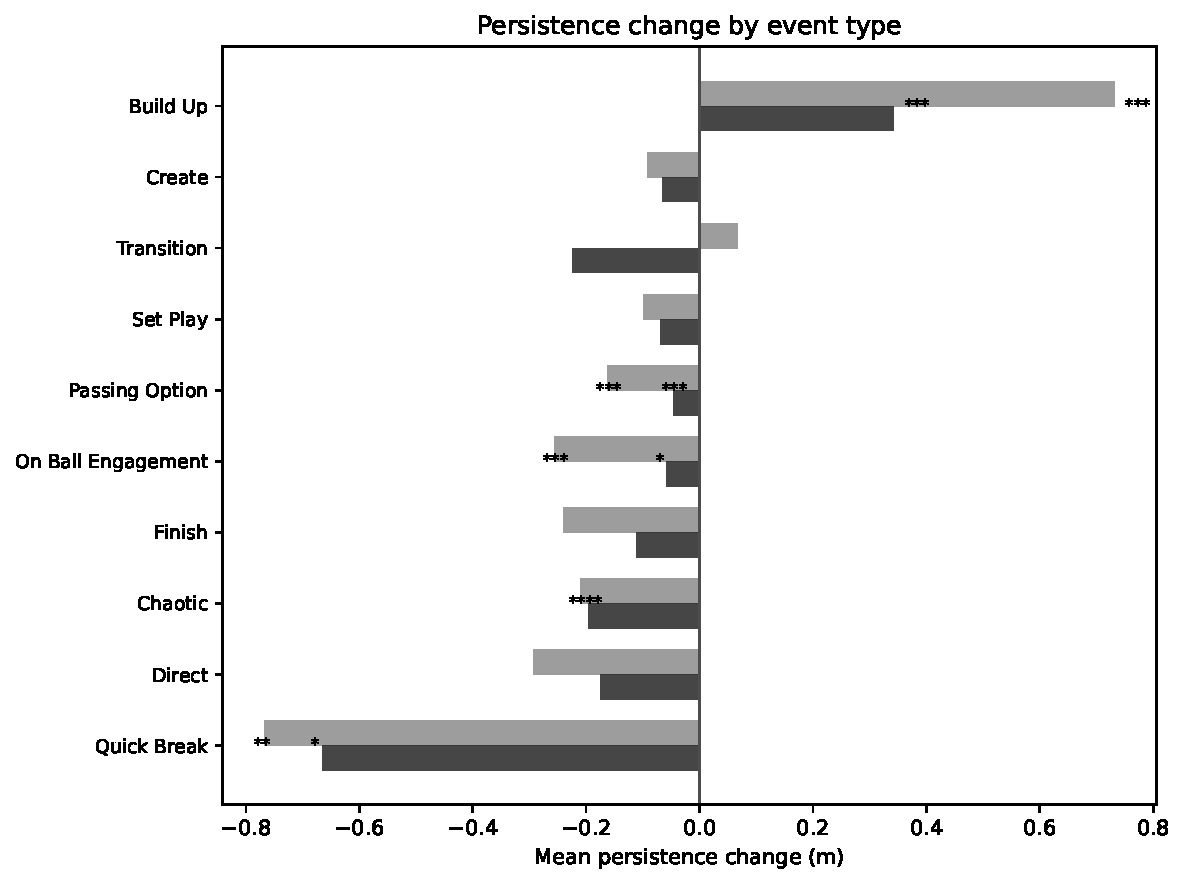
\includegraphics[width=\textwidth]{figures/fig_event_correlation}
\caption{Mean persistence change ($\Delta p$) by event type for individual (grey) and tactical (dark) scales. Bars show mean values. Significance markers above each bar indicate FDR-corrected Mann--Whitney $U$ test results (*** $p<0.001$; ** $p<0.01$; * $p<0.05$). Events are sorted left to right from strongest negative (disruption) to strongest positive (organisation) effect.}
\label{fig:events}
\end{figure}

\begin{table}
\tbl{Window-sensitivity check: direction and significance of persistence change by event window width ($\pm$ seconds). Individual scale shown; tactical scale shows the same directional pattern throughout.}
{\begin{tabular}{lcccccc} \toprule
 & \multicolumn{2}{c}{$\pm 0.5$~s} & \multicolumn{2}{c}{$\pm 1$~s} & \multicolumn{2}{c}{$\pm 5$~s} \\
\cmidrule(lr){2-3}\cmidrule(lr){4-5}\cmidrule(lr){6-7}
Event type & Direction & Sig. & Direction & Sig. & Direction & Sig. \\ \midrule
On-ball engagement & negative & *** & negative & *** & negative & *** \\
Passing option     & negative & *** & negative & *** & negative & *** \\
Build-up phase     & positive & *** & positive & *** & positive & *** \\
Quick break        & negative & *   & negative & *   & negative & ns  \\
Chaotic phase      & negative & *   & negative & *   & negative & ns  \\
\bottomrule
\end{tabular}}
\tabnote{Direction of mean persistence change is identical across all three window widths for all five event types. Significance drops to ns at $\pm5$~s for quick break and chaotic phase due to smaller sample sizes ($n=57$ and $n=1{,}052$ respectively) and dilution by surrounding play. *** $p<0.001$; * $p<0.05$; ns not significant.}
\label{tab:windows}
\end{table}

\subsection{Topology versus Standard Geometric Descriptors}

Coaches and analysts already track team shape using simple geometric
measures: how long and wide a team is, how much pitch area its outline
encloses, and how evenly its players are spread (team length, team
width, convex-hull area, and Voronoi dispersion entropy). This analysis
asks whether tactical-scale topological persistence is simply a
restatement of one of these measures, or whether it adds something they
miss. Across the ten-match sample, persistence correlated weakly with
team width and convex-hull area, and barely at all with team length
(Table~\ref{tab:baseline}); the correlations were statistically
significant but modest in size, reflecting the large number of frames
analysed rather than a strong relationship. After accounting for all
three geometric measures together, tactical-scale persistence still
explained a meaningful share of the variation left over, most notably for
convex-hull area, the closest of the four to what persistence is
actually measuring.

The practical reading is that persistence is not a relabelled version
of any existing geometric measure: it tracks something the standard
descriptors do not fully capture, even though the relationship between
them is loose rather than independent. This is a correlational result,
established within the present sample; the next analysis asks the
stronger question of whether that extra information actually helps
predict what is happening in a match.

\begin{table}
\tbl{Tactical-scale persistence versus geometric baseline descriptors (10 matches, 1{,}500 frames).}
{\begin{tabular}{lccc} \toprule
Descriptor & Spearman $\rho$ & $p$ & Partial $R^2$ \\ \midrule
Team length & $-0.005$ & $0.857$ & $0.025$ \\
Team width & $0.356$ & $<10^{-40}$ & $0.036$ \\
Convex-hull area & $0.431$ & $<10^{-65}$ & $0.091$ \\
Voronoi dispersion entropy & $0.126$ & $9.9\times10^{-7}$ & $0.004$ \\
\bottomrule
\end{tabular}}
\label{tab:baseline}
\end{table}

\subsection{Home and Away Tactical Independence}

Splitting the analysis by team, rather than merging both sides into one
22-player cloud, asks a different question: do a team's own
tactical-scale formations relate to its opponent's, or does each side
organise independently? Running the pipeline separately on each team's
11 players roughly doubles the rate at which tactical-scale loops
appear compared with the merged analysis (around 36\% of frames per
team, versus 19\% in the merged view), simply because splitting by team
gives the underlying clustering twice as many points to work with
(Table~\ref{tab:bilateral}).

Whether one team's tactical persistence tracks the other's is a
separate question from how often each shows a loop at all, and the
answer here is that it largely does not. Home and away tactical
persistence correlated only weakly with each other, and the same weak
relationship held whether we compared the two teams at the same moment
or allowed for a short delay of up to a second in either direction
(Table~\ref{tab:coupling}). Both teams showed a loop in the same frame
only slightly more often than chance would predict.

For analysis purposes, this means a team's tactical shape can be read
largely on its own terms: at this temporal resolution, what one side is
doing structurally is not a strong signal of what the other is doing,
and the two should be assessed independently rather than assumed to be
coupled.

\begin{table}
\tbl{Per-team tactical-scale $H_1$ statistics (10 matches, 1{,}500 frames).}
{\begin{tabular}{lccc} \toprule
Sub-cloud & Mean tactical clusters & $H_1$ presence rate & Mean $H_1$ total persistence \\ \midrule
Home (11 players) & $5.27\pm2.28$ & $36.1\%$ & 1.535 \\
Away (11 players) & $5.21\pm2.39$ & $36.4\%$ & 1.552 \\
22-player merged (reference) & $4.92\pm0.36$ & $19.3\%\pm7.2\%$ & --- \\
\bottomrule
\end{tabular}}
\tabnote{Home and away rows are from the bilateral decomposition in this study. The 22-player merged reference row reports tactical-scale cluster count and $H_1$ presence from the companion methodological paper \cite{paperA}.}
\label{tab:bilateral}
\end{table}

\begin{table}
\tbl{Cross-team coupling at the tactical scale (10 matches, 1{,}500 frames).}
{\begin{tabular}{lc} \toprule
Quantity & Value \\ \midrule
Cross-team Spearman $\rho$ (lag 0) & $0.037$ [$-0.018$, $0.087$] \\
Cross-team Spearman $\rho$ (lag $\pm1$ frame) & $\in[-0.048,-0.013]$ \\
Cross-team Spearman $\rho$ (lag $\pm5$ frames) & $\in[-0.057,-0.040]$ \\
Co-occurrence $P(\text{both teams } H_1>0)$ & $14.7\%$ \\
Co-occurrence $P(\text{neither team})$ & $42.1\%$ \\
\bottomrule
\end{tabular}}
\label{tab:coupling}
\end{table}

\begin{figure}
\centering
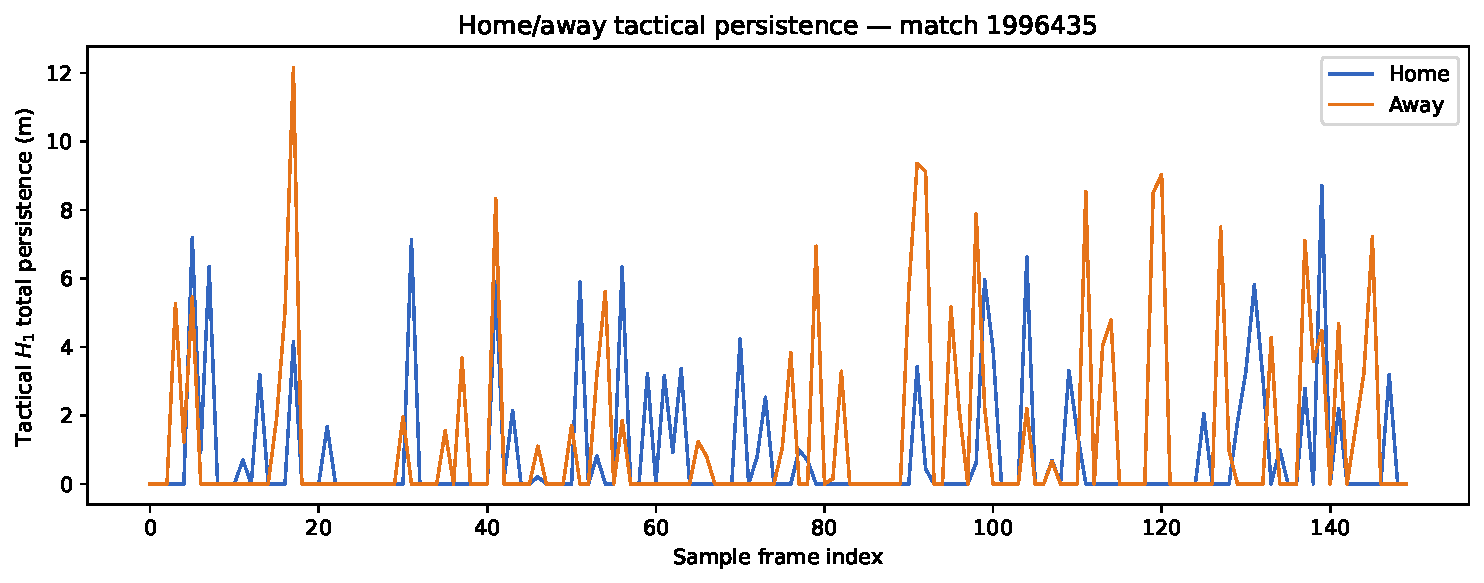
\includegraphics[width=\textwidth]{figures/fig_bilateral_timeseries}
\caption{Home (blue) and away (orange) tactical-scale $H_1$ total persistence over the 150 uniformly sampled frames of the primary match (SkillCorner ID 1996435). The merged 22-player series (grey) is shown for reference. The two team series evolve largely independently (Spearman $\rho = 0.037$; Table~\ref{tab:coupling}).}
\label{fig:bilateral}
\end{figure}

\subsection{Predictive Value for Phase-of-Play Classification}

The previous analysis showed that tactical-scale persistence carries
information the geometric descriptors do not, within the sample
analysed. The practical question for an analyst is sharper: does adding
that information actually improve a prediction made on a match the
model has never seen? We tested this directly, training a classifier to
detect build-up phases from frame-level features, with every match held
out of training in turn, measuring performance always on
unseen matches. The four geometric descriptors alone already predicted
build-up phases reasonably well (Table~\ref{tab:predictive}). Adding tactical-scale persistence, whether as total persistence, loop count, or maximum persistence, did not improve that prediction; if anything,
performance was marginally and not significantly worse. The same null
result held for a second target, chaotic phases.

The honest reading is that, on the present ten-match sample,
tactical-scale persistence does not yet earn its place as a predictive
feature alongside measures coaches already use, even though the
previous analysis showed it carries non-redundant information in
principle. The most likely explanation is sample size rather than a
genuine absence of signal: with only ten matches to estimate a single
new feature's contribution, there may simply not be enough data for
that contribution to show up reliably in held-out performance. Settling
this will require the larger, population-scale dataset described in
the companion full-season work.

\begin{table}
\tbl{Cross-validated predictive performance for build-up phase classification (10 matches, 1{,}500 frames).}
{\begin{tabular}{lccc} \toprule
Topology summary added & AUC (with / without) & $\Delta$AUC [95\% CI] & Permutation $p$ \\ \midrule
Tactical $H_1$ total persistence & $0.687$ / $0.693$ & $-0.005$ [$-0.015$, $+0.001$] & $1.00$ \\
Tactical $H_1$ count & $0.689$ / $0.693$ & $-0.004$ [$-0.010$, $+0.0004$] & $1.00$ \\
Tactical $H_1$ max persistence & $0.687$ / $0.693$ & $-0.006$ [$-0.016$, $+0.001$] & $1.00$ \\
\bottomrule
\end{tabular}}
\label{tab:predictive}
\end{table}

\begin{figure}
\centering
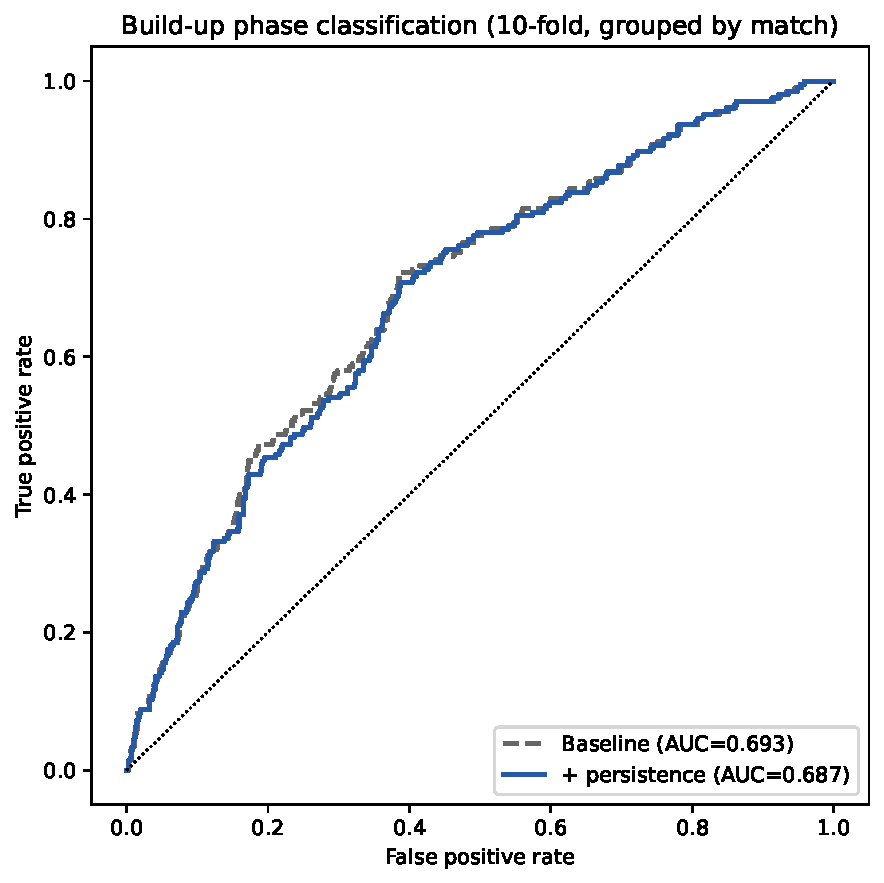
\includegraphics[width=0.7\textwidth]{figures/fig_roc_overlay}
\caption{ROC curves for build-up phase classification using the geometric descriptor baseline (dashed, AUC $= 0.693$) and geometric descriptors plus tactical-scale $H_1$ total persistence (solid, AUC $= 0.687$). Curves are built from out-of-fold predicted probabilities under match-grouped ten-fold cross-validation. The two curves are nearly overlapping, consistent with the null result in Table~\ref{tab:predictive}.}
\label{fig:roc}
\end{figure}
